% =====================================================================
% 03_results.tex  --  Results, observations, critical analysis (Exp. 4)
% =====================================================================

\section{Results}
\label{sec:dproxy-results}

\subsection{The contrastive adjustment does not selectively suppress hallucinations}
\label{subsec:dproxy-res-d}

Table~\ref{tab:dproxy-top10} reports $d = E - A$ over the expert's top-10 object
candidates at each step. We use the candidate set rather than only the emitted
word because it is not conditioned on a token winning, so it carries no selection
effect. The finding is clearest on Qwen and weaker but consistent on LLaVA, and
we state it precisely rather than as a blanket claim.

On Qwen the adjustment is negative overall, meaning the method lowers object
logits, but it lowers \emph{real} objects far more than hallucinations (VCD mean
$-0.984$ for real versus $-0.429$ for hallucinated; SID $-0.674$ versus
$-0.172$), and the share of amplified tokens is higher for hallucinations
($36.1\%$ versus $25.1\%$ under VCD). This is the opposite of the intended
behaviour and it holds at every window. On LLaVA the adjustment is small in
magnitude for both groups and its ordering is not stable: under VCD hallucinated
$d$ is marginally above real ($+0.164$ versus $+0.133$), while under SID it is
below real ($+0.114$ versus $+0.218$), with both groups amplified rather than
suppressed. The LLaVA-SID row is the only one of the four in which hallucinated
$d$ sits below real $d$, which is the direction H1 predicts; we return to it
below, because it does not survive the other two views.

\begin{table}[t]
\centering
\small
\setlength{\tabcolsep}{5pt}
\caption{\textbf{Contrastive adjustment $d = E - A$ over the expert's top-10
object candidates.} Mean of $d$ and the percentage of tokens with $d > 0$ (the
share amplified rather than suppressed), for real and hallucinated objects.}
\label{tab:dproxy-top10}
\begin{tabular}{ll cc cc}
\toprule
& & \multicolumn{2}{c}{Real objects} & \multicolumn{2}{c}{Hallucinated objects} \\
\cmidrule(lr){3-4}\cmidrule(lr){5-6}
Model & Method & mean $d$ & \% $d\!>\!0$ & mean $d$ & \% $d\!>\!0$ \\
\midrule
LLaVA-1.5-7B & VCD & $+0.133$ & $56.9$ & $+0.164$ & $57.2$ \\
 & SID & $+0.218$ & $59.3$ & $+0.114$ & $50.3$ \\
Qwen2.5-VL-7B & VCD & $-0.984$ & $25.1$ & $-0.429$ & $36.1$ \\
 & SID & $-0.674$ & $31.9$ & $-0.172$ & $41.6$ \\
\bottomrule
\end{tabular}
\end{table}

Figures~\ref{fig:dproxy-llava} and~\ref{fig:dproxy-qwen} show the full per-token
spread over the top-10 candidates. Red bars are tokens contrastive decoding
amplifies ($d > 0$), blue bars are tokens it suppresses ($d < 0$), and the dashed
line is the group mean. On Qwen the real-object panels are markedly more negative
than the hallucination panels, which is the visual form of the numbers above.

\begin{figure}[t]
\centering
\begin{minipage}{0.49\linewidth}\centering
  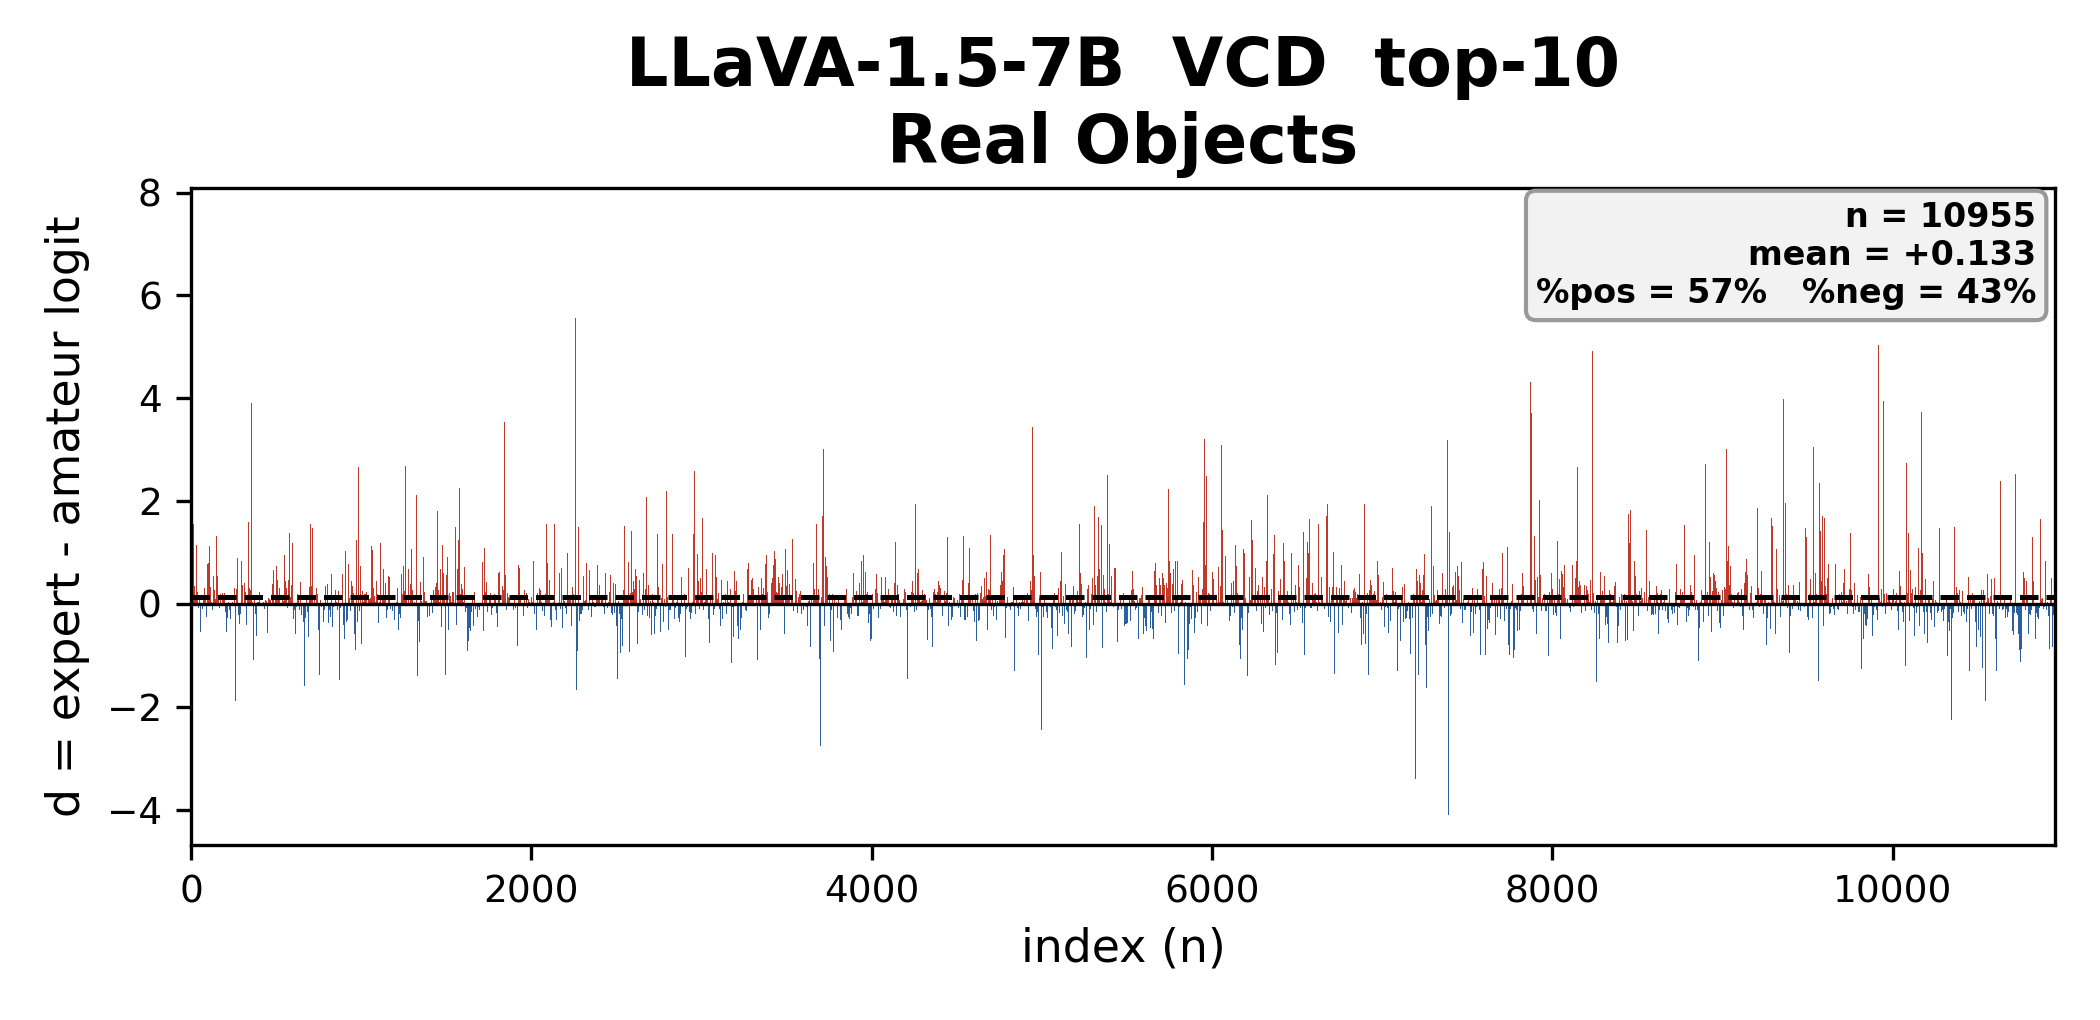
\includegraphics[width=\linewidth]{figs/llava_top10_vcd_real.png}\\[-1pt]
  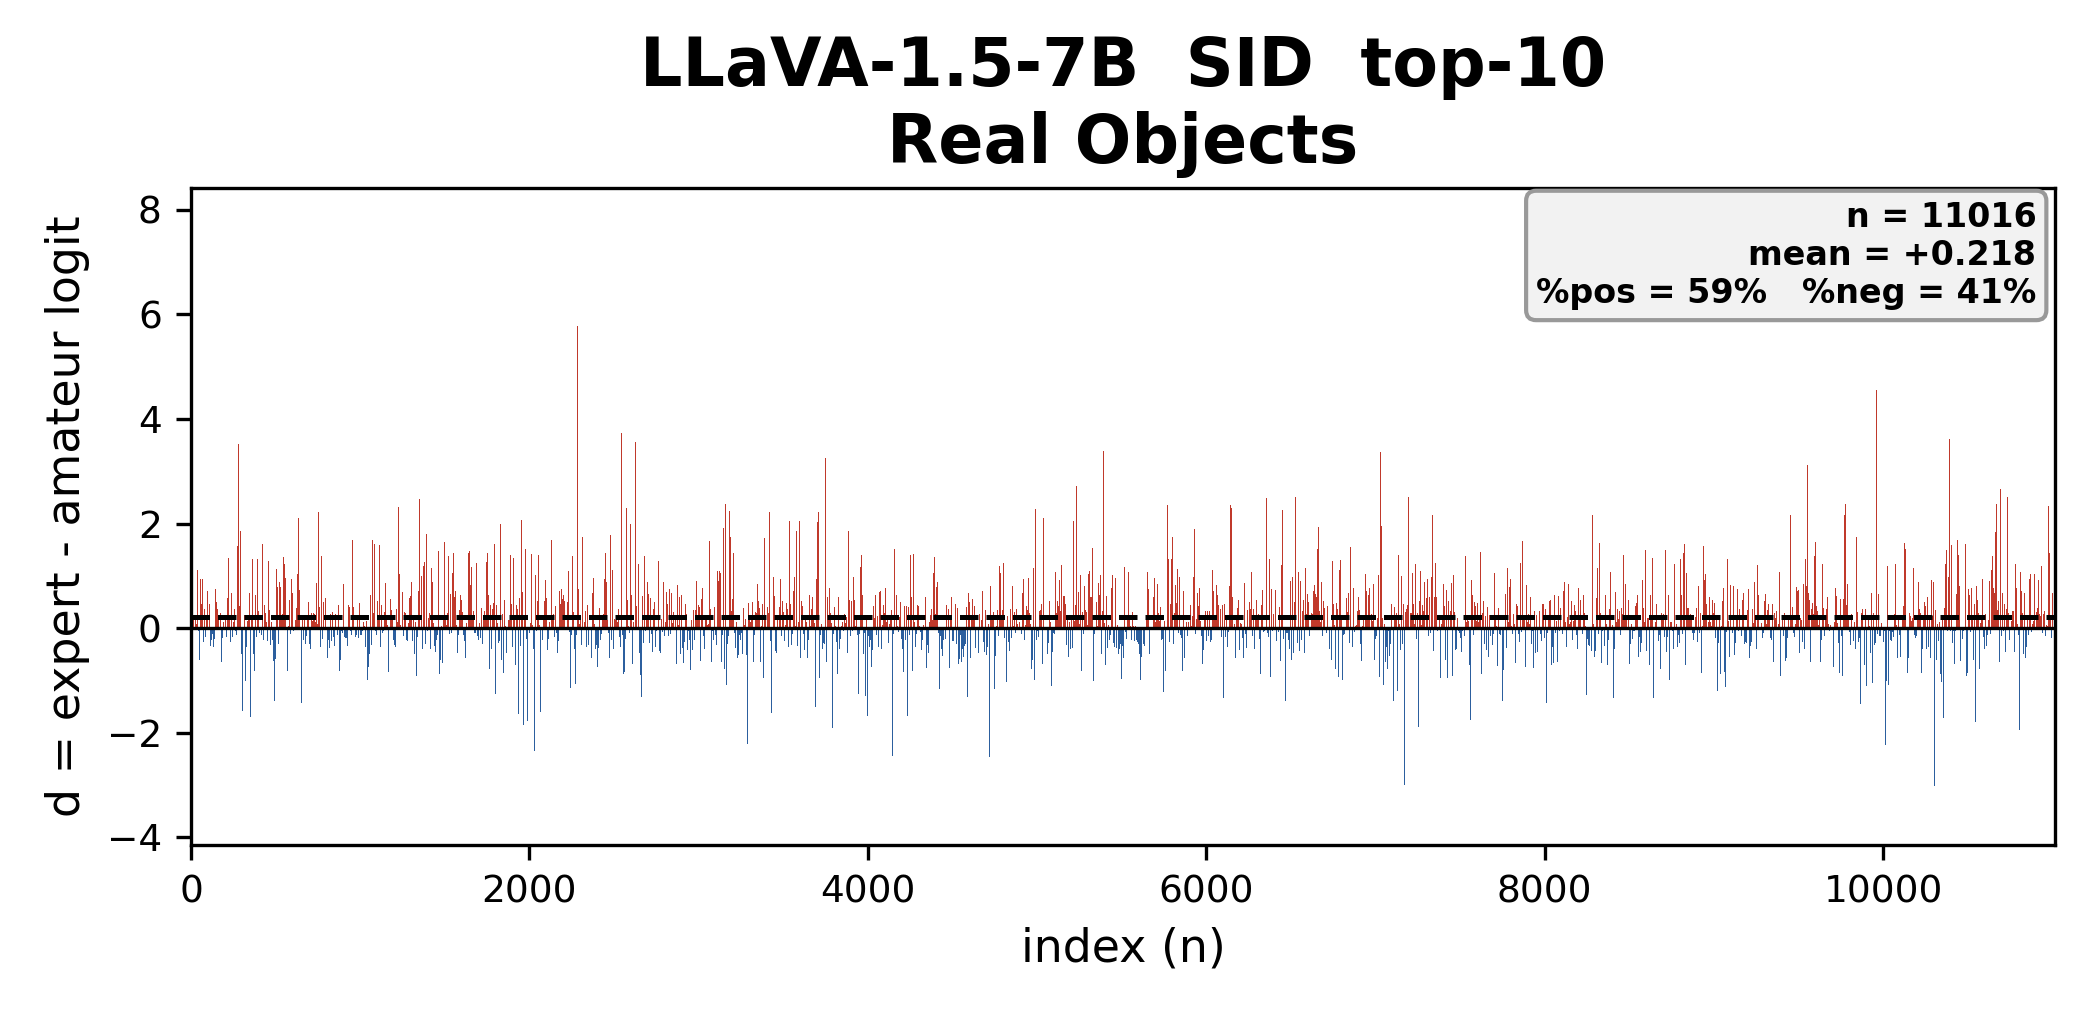
\includegraphics[width=\linewidth]{figs/llava_top10_sid_real.png}
\end{minipage}\hfill
\begin{minipage}{0.49\linewidth}\centering
  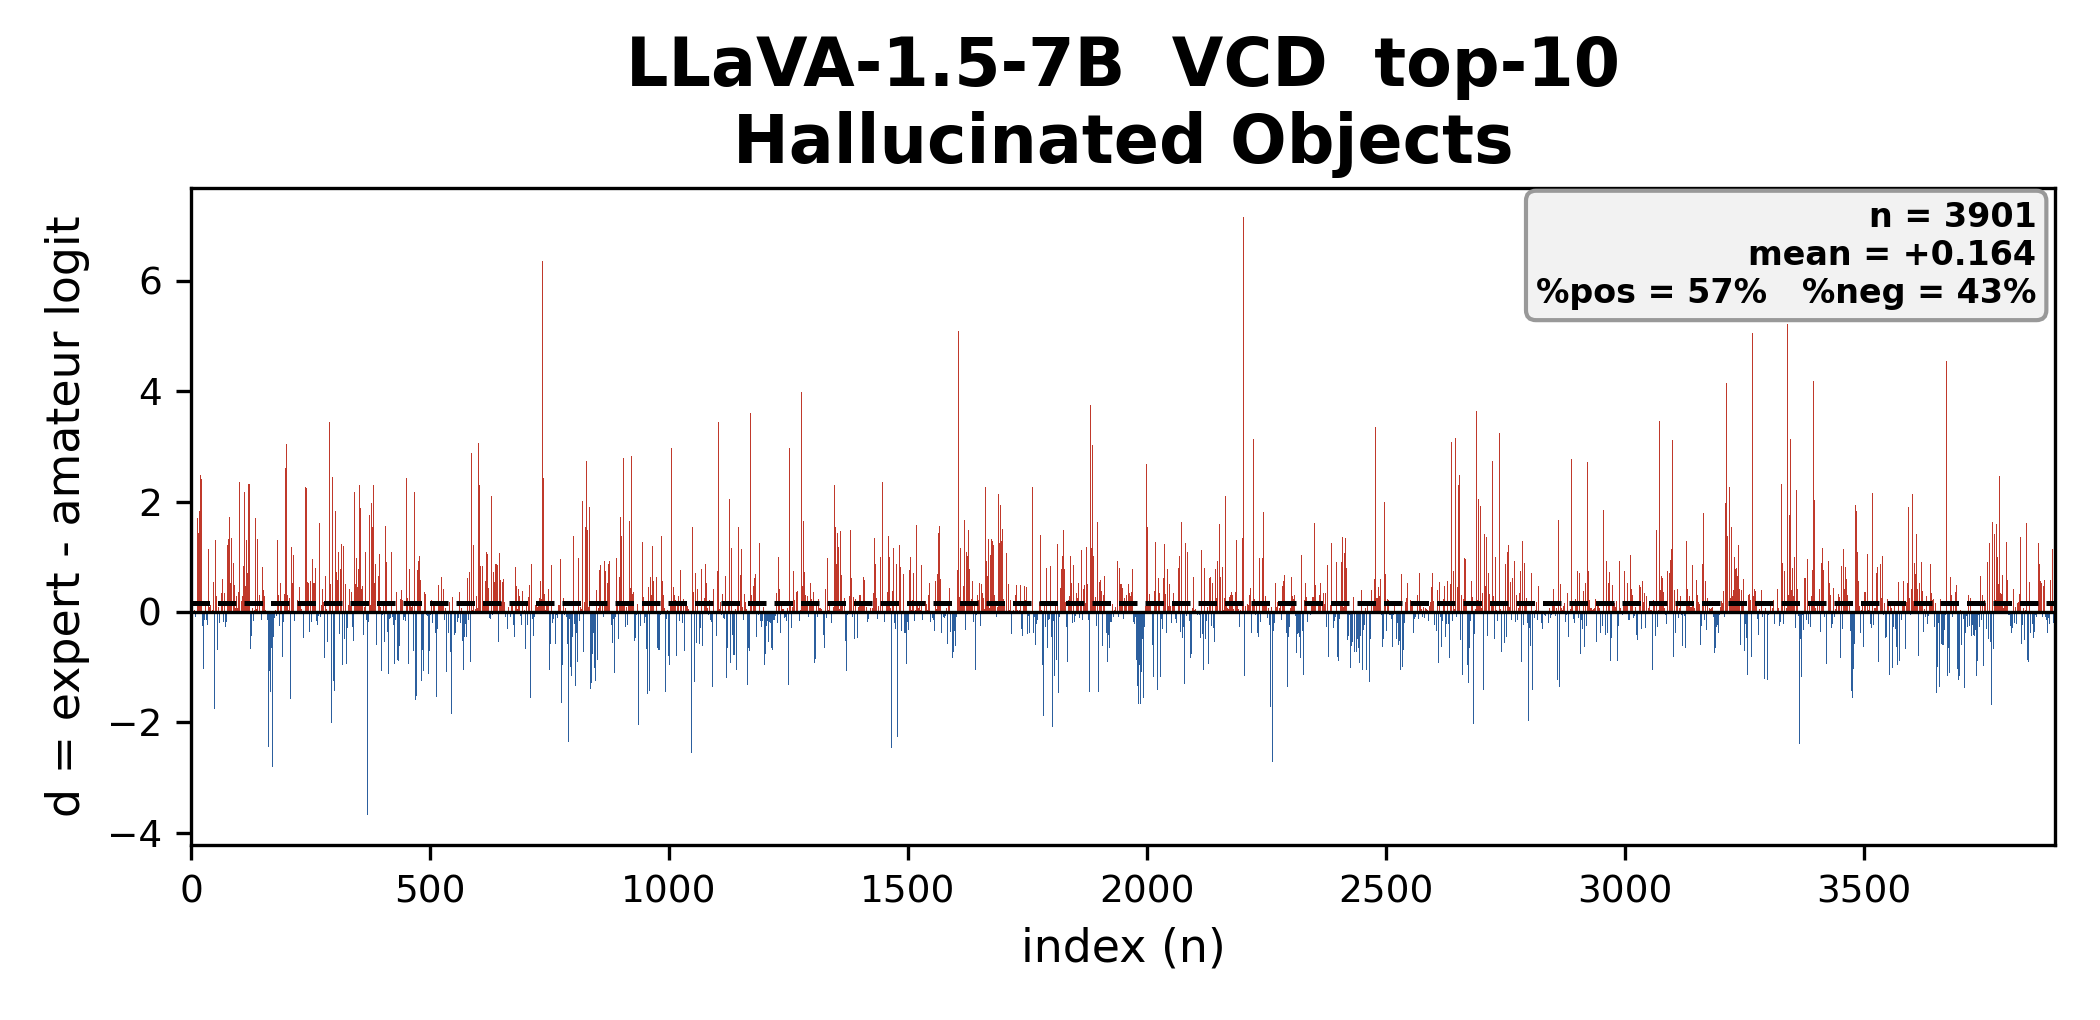
\includegraphics[width=\linewidth]{figs/llava_top10_vcd_hall.png}\\[-1pt]
  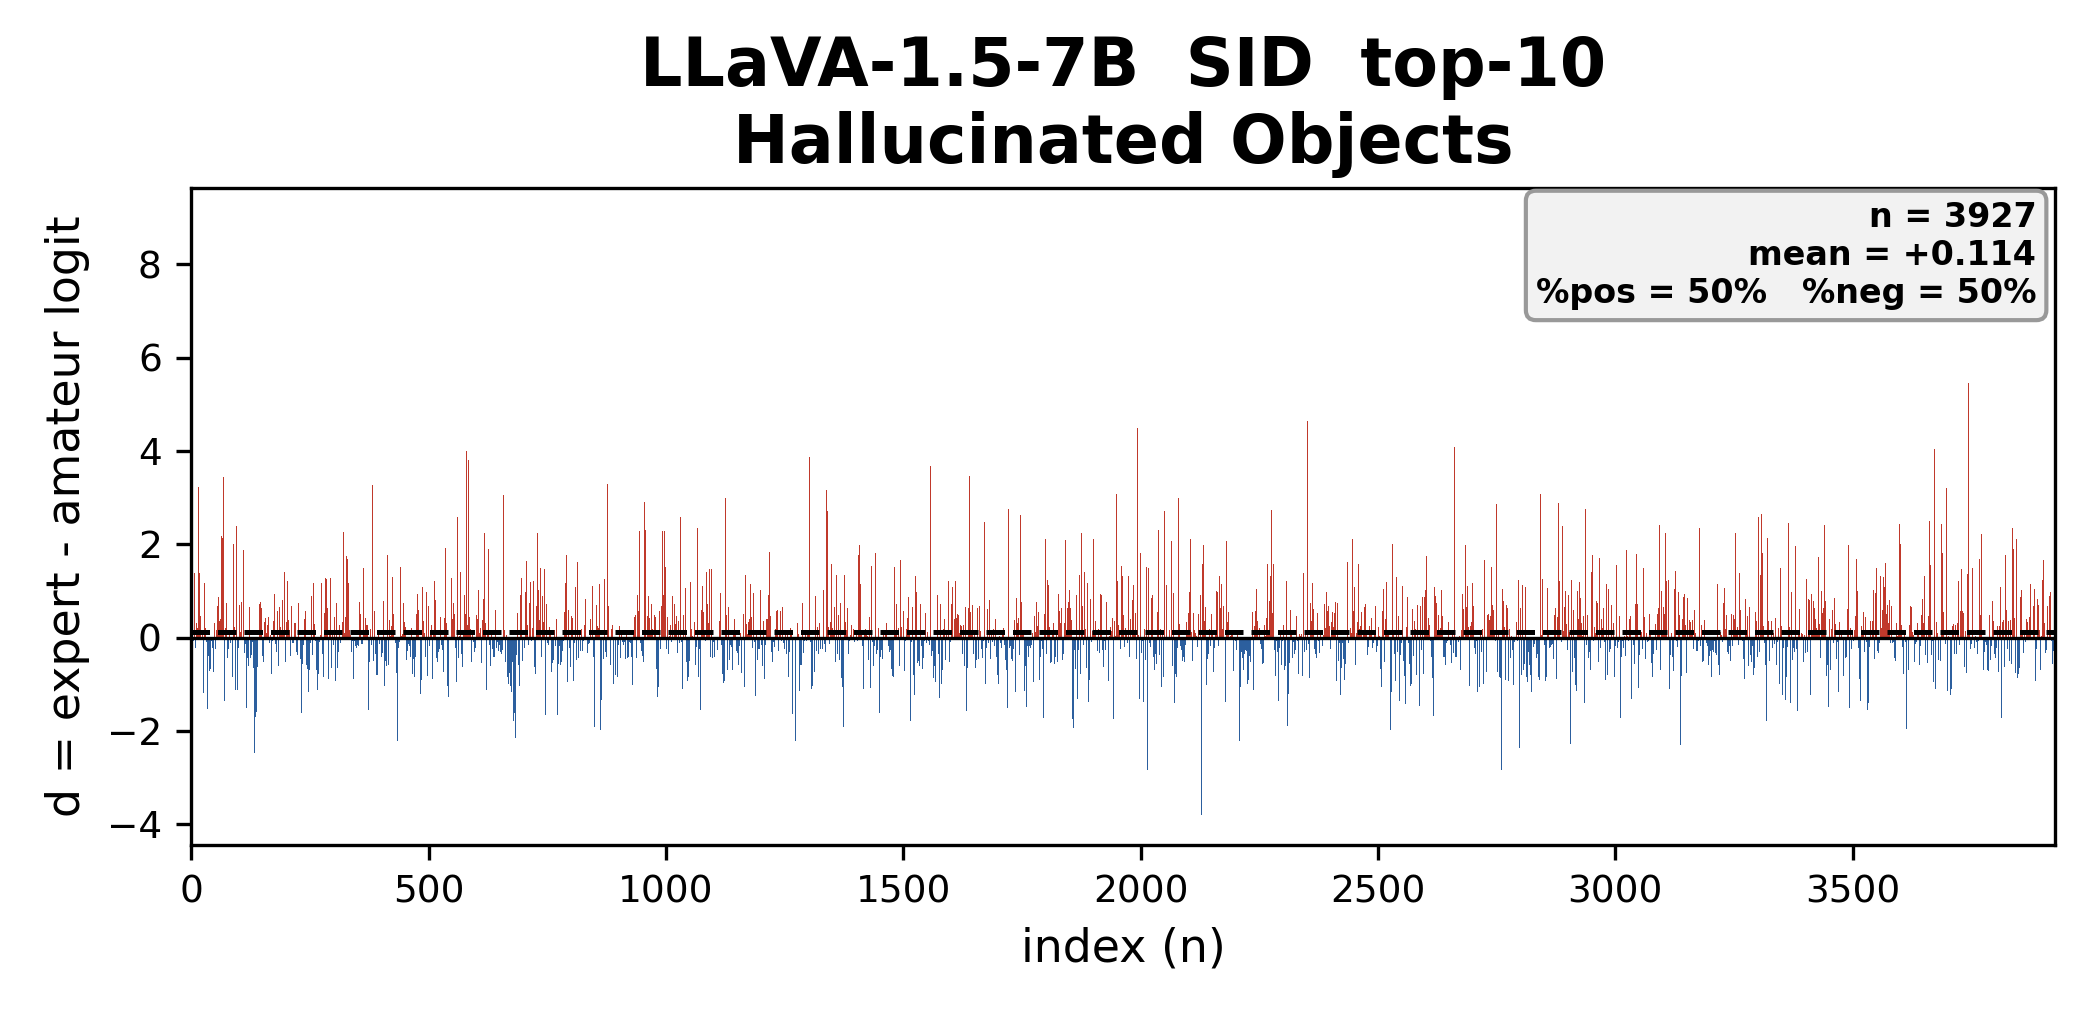
\includegraphics[width=\linewidth]{figs/llava_top10_sid_hall.png}
\end{minipage}
\caption{\textbf{LLaVA-1.5-7B: $d = E - A$ over top-10 object candidates.} Left
column real objects, right column hallucinated objects; top row VCD, bottom row
SID. The adjustment is positive (amplifying) and small for both groups.}
\label{fig:dproxy-llava}
\end{figure}

\begin{figure}[t]
\centering
\begin{minipage}{0.49\linewidth}\centering
  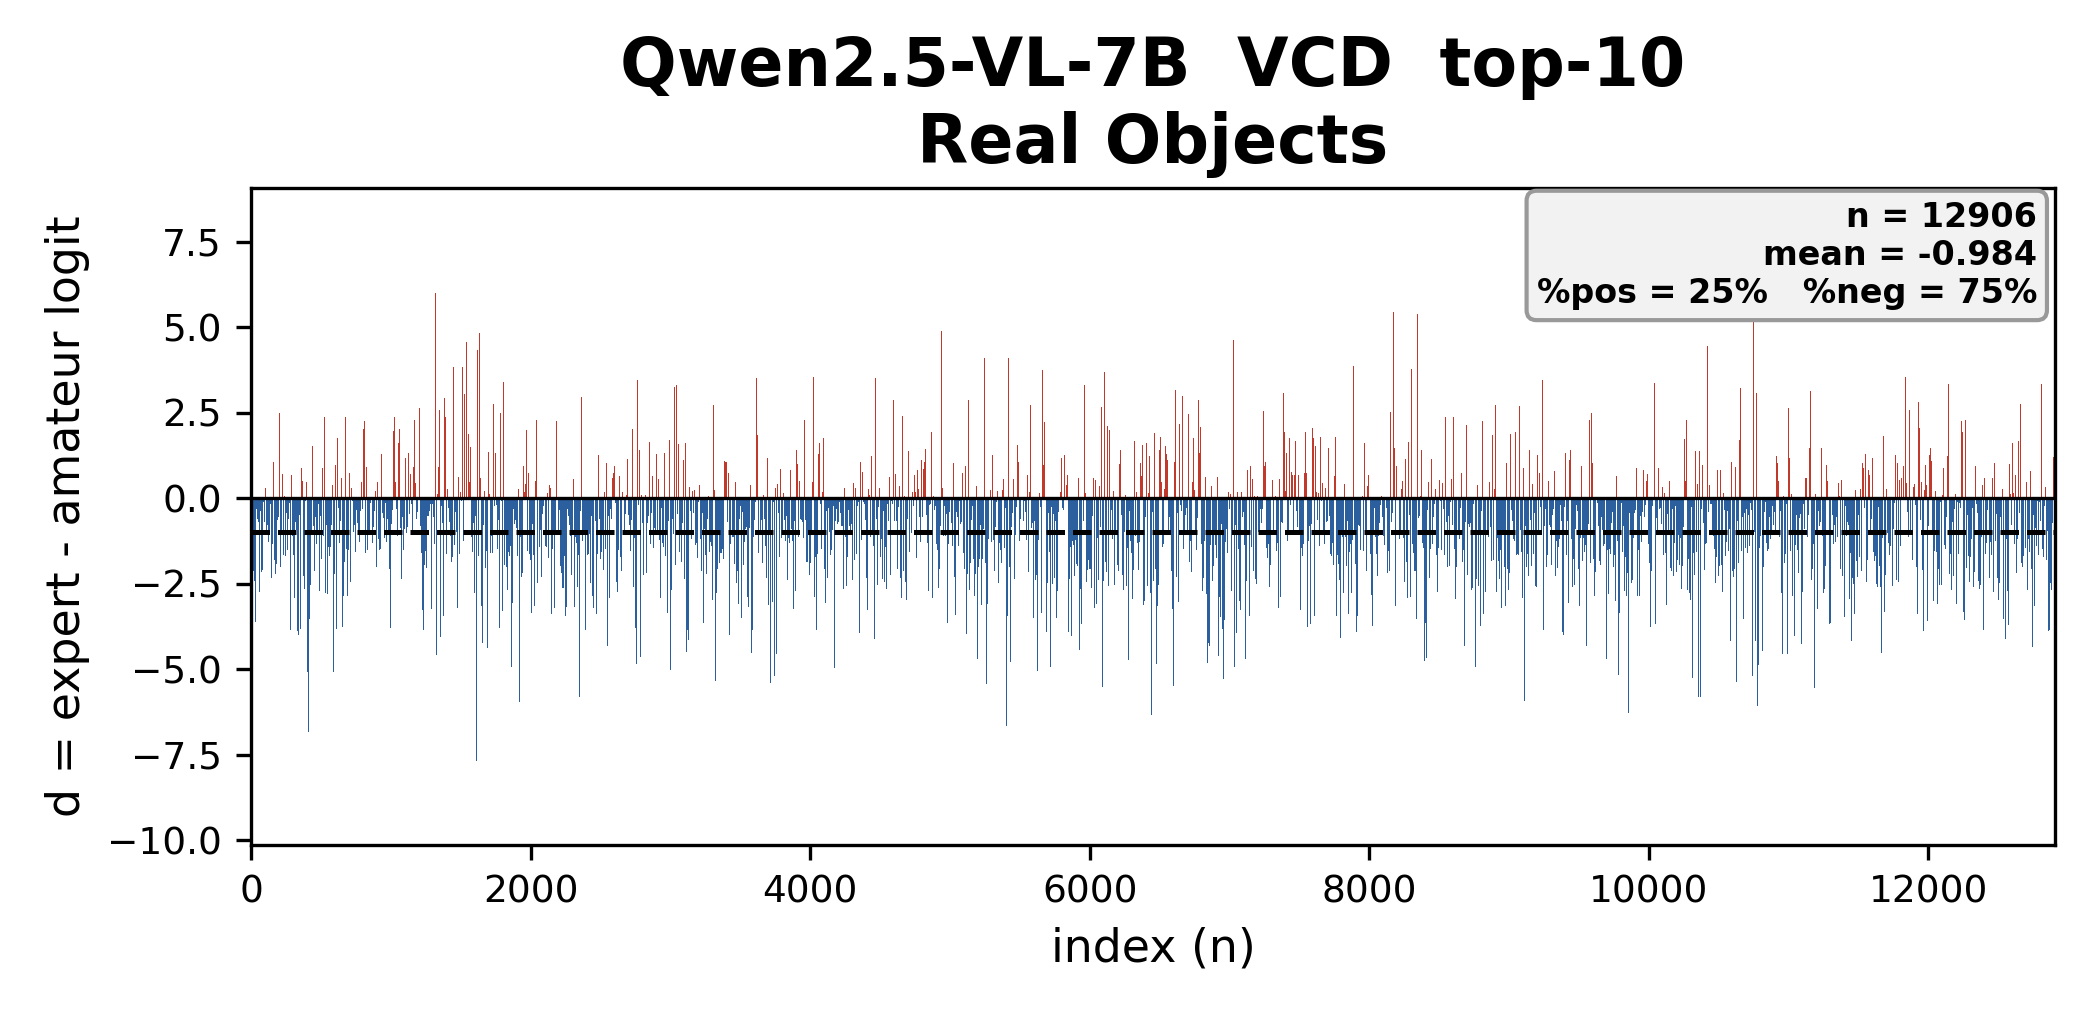
\includegraphics[width=\linewidth]{figs/qwen_top10_vcd_real.png}\\[-1pt]
  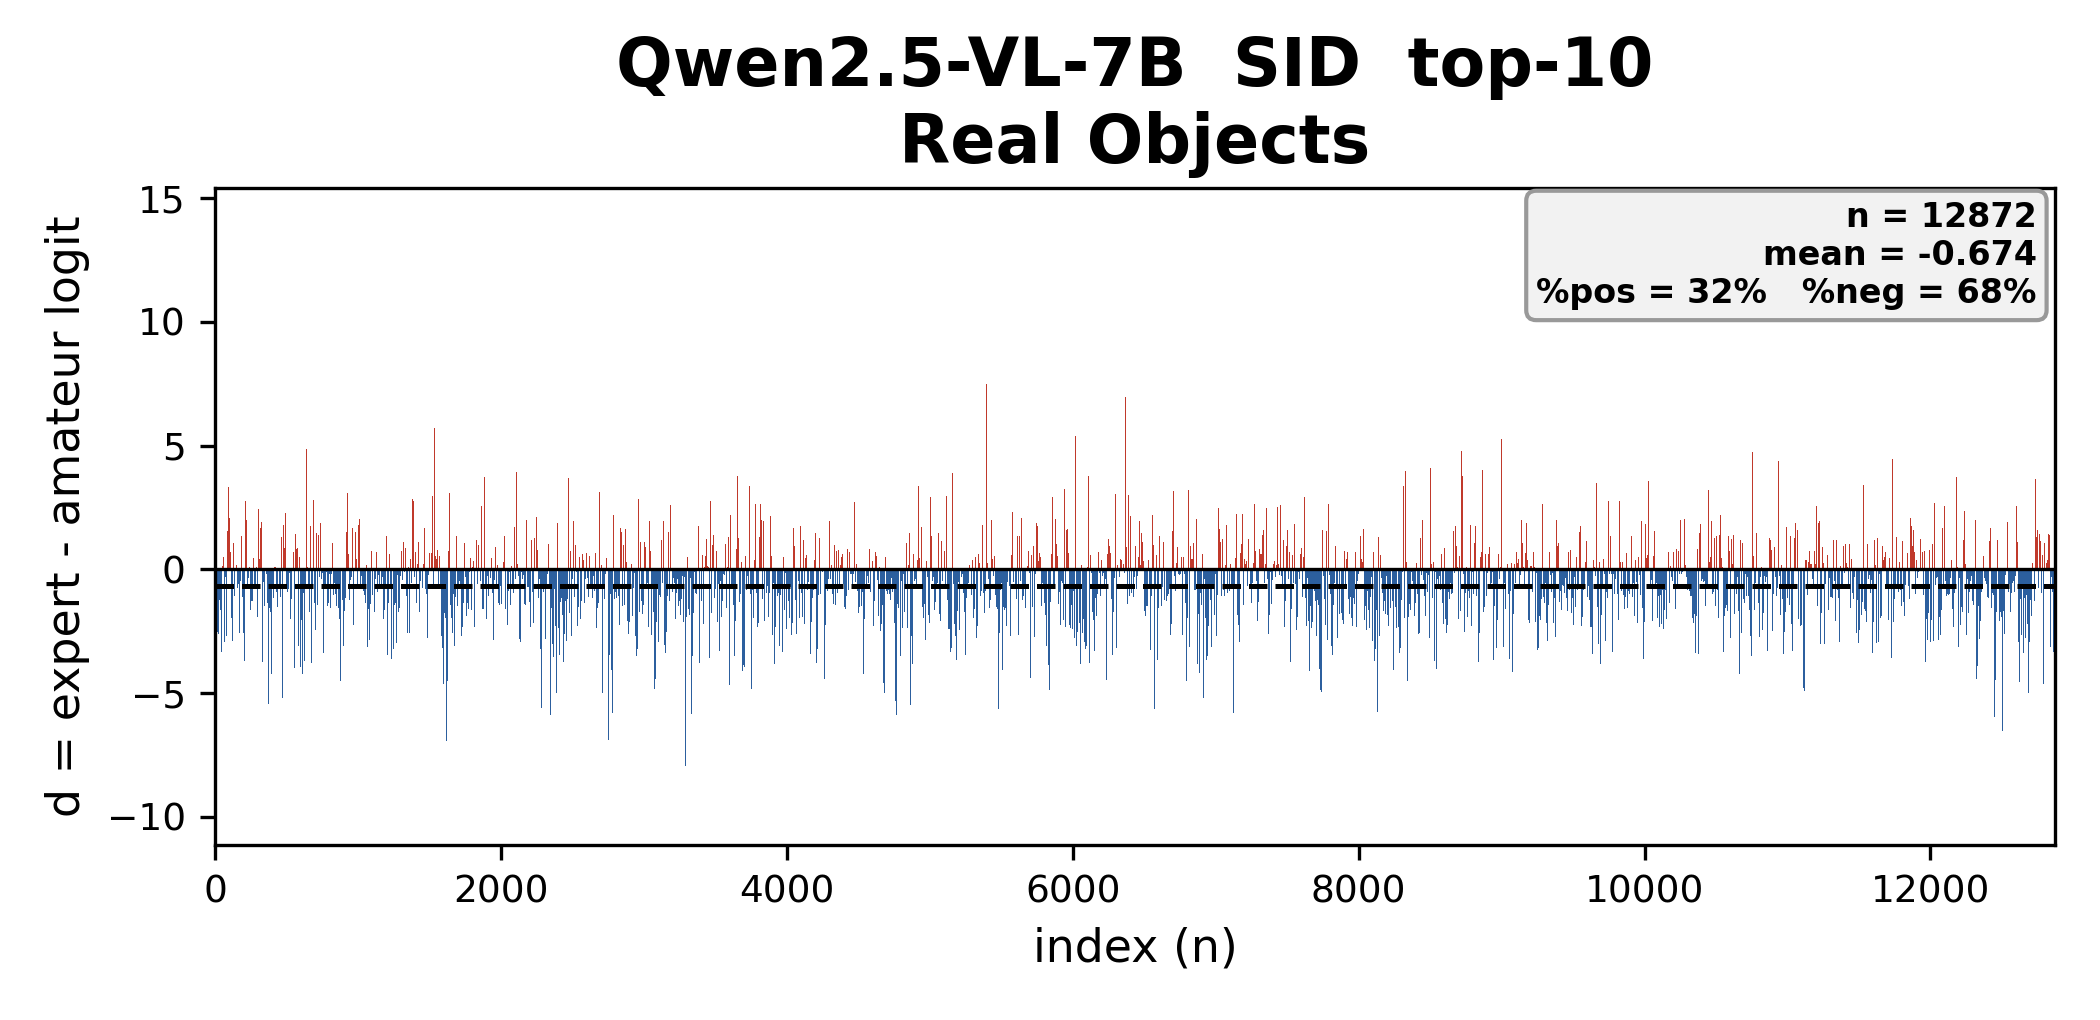
\includegraphics[width=\linewidth]{figs/qwen_top10_sid_real.png}
\end{minipage}\hfill
\begin{minipage}{0.49\linewidth}\centering
  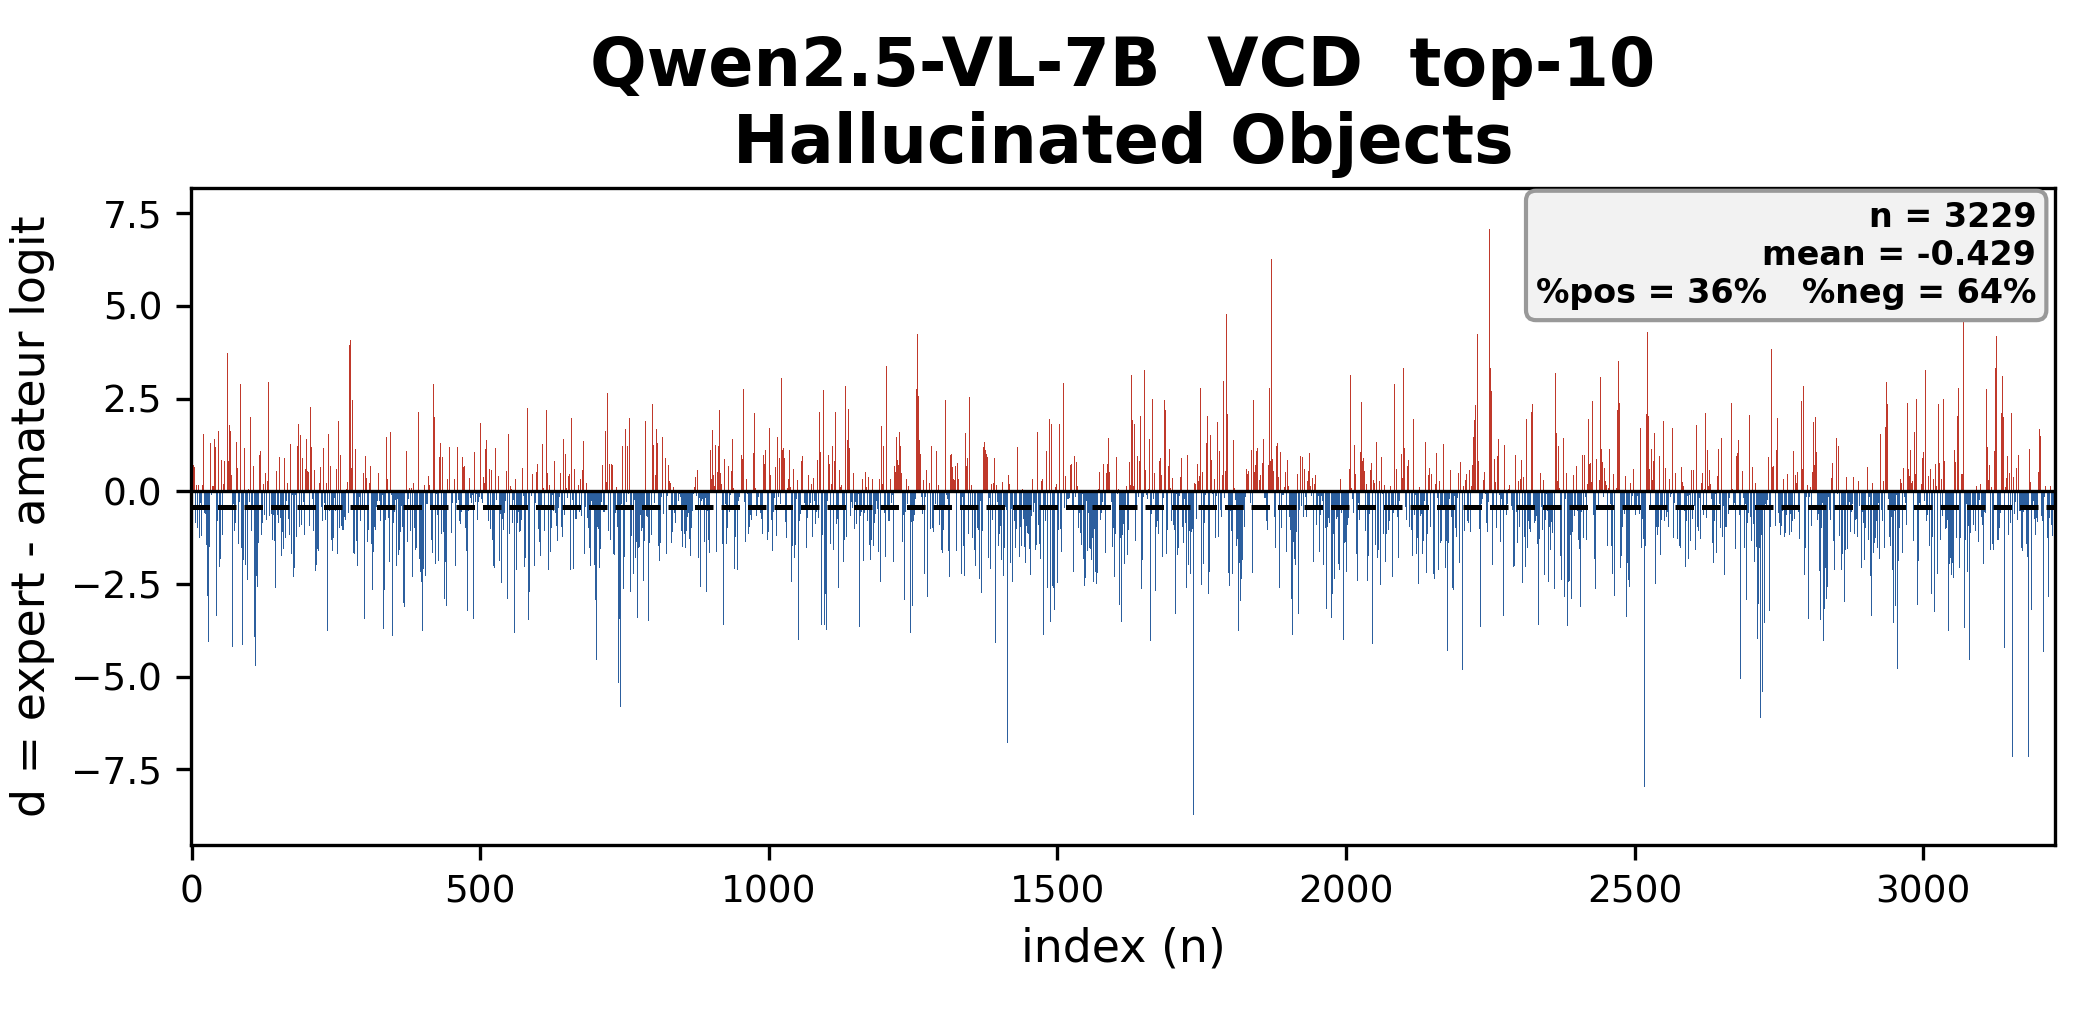
\includegraphics[width=\linewidth]{figs/qwen_top10_vcd_hall.png}\\[-1pt]
  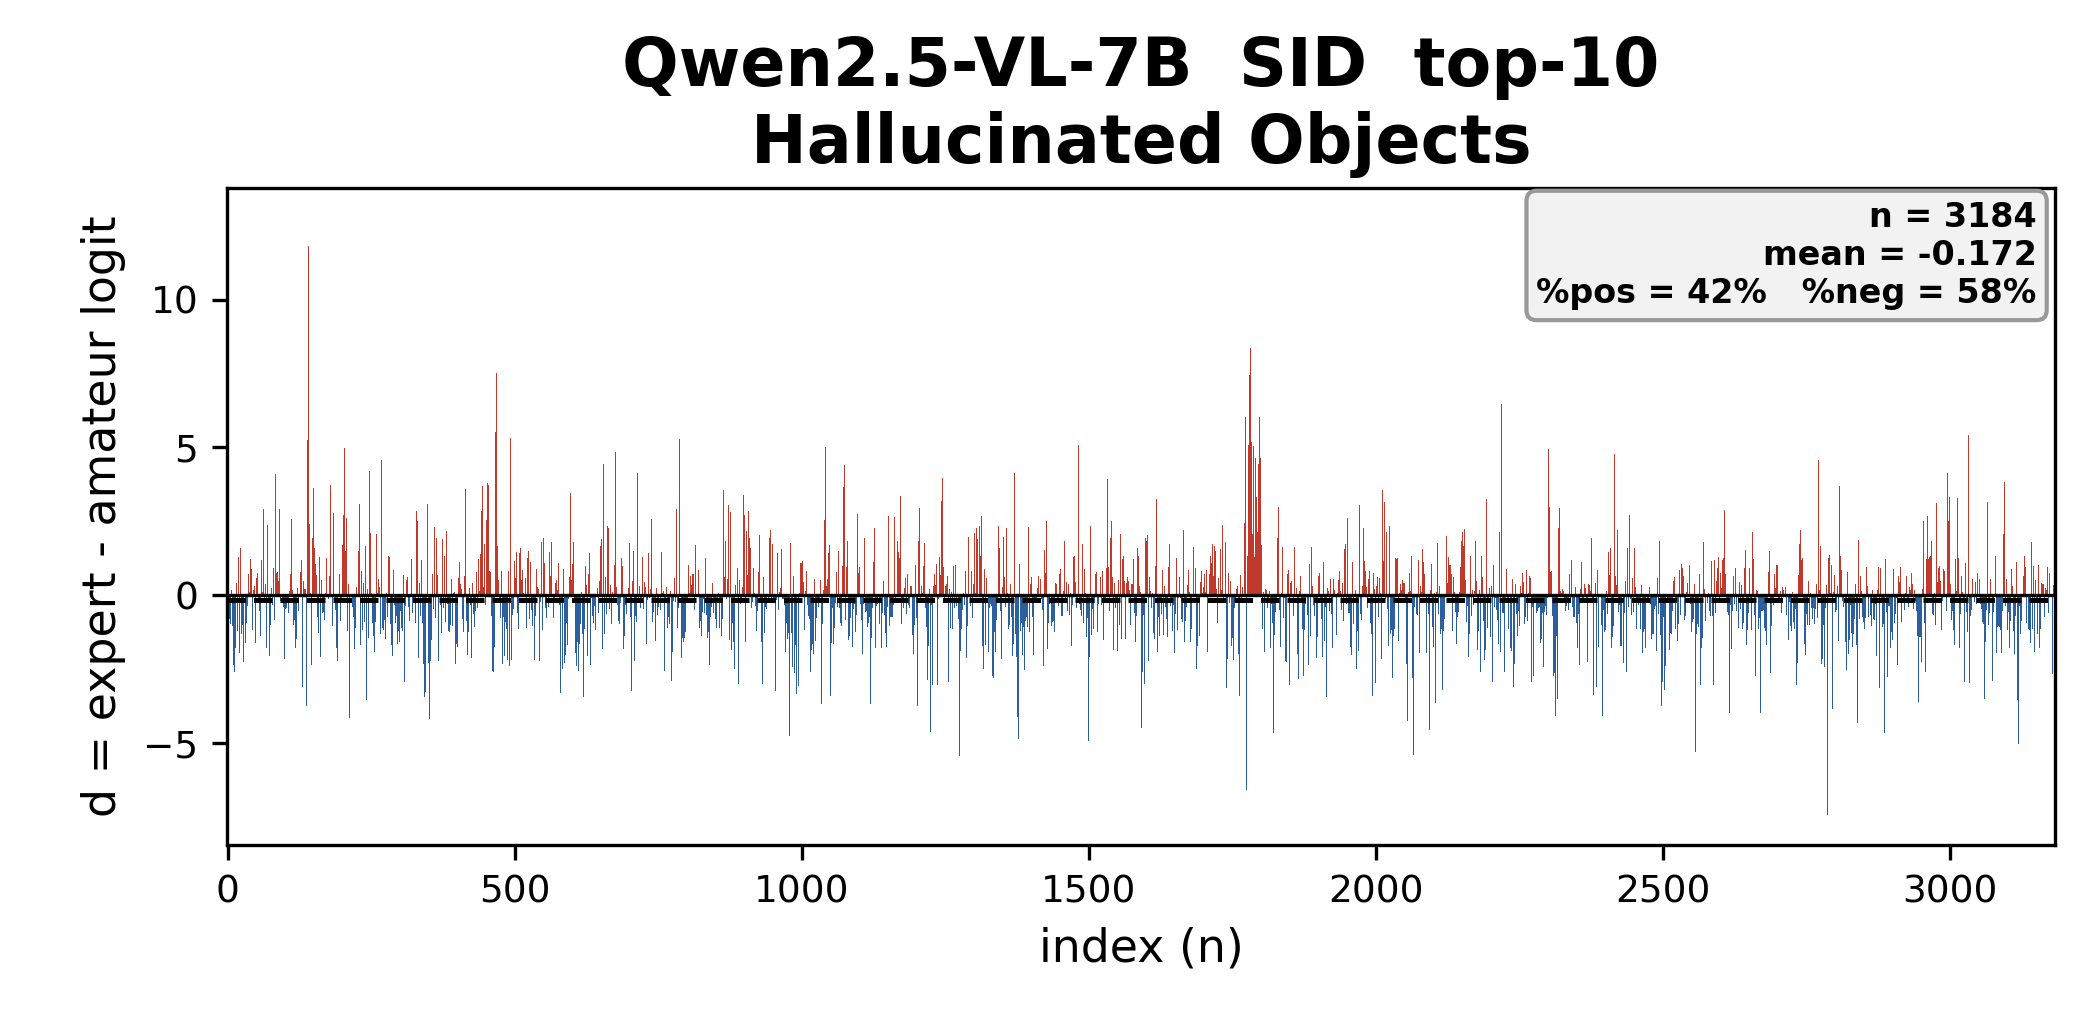
\includegraphics[width=\linewidth]{figs/qwen_top10_sid_hall.png}
\end{minipage}
\caption{\textbf{Qwen2.5-VL-7B: $d = E - A$ over top-10 object candidates.} Layout
as in Figure~\ref{fig:dproxy-llava}. Real objects are suppressed more than
hallucinations, the opposite of the intended behaviour.}
\label{fig:dproxy-qwen}
\end{figure}

\begin{figure}[t]
\centering
\begin{minipage}{0.49\linewidth}\centering
  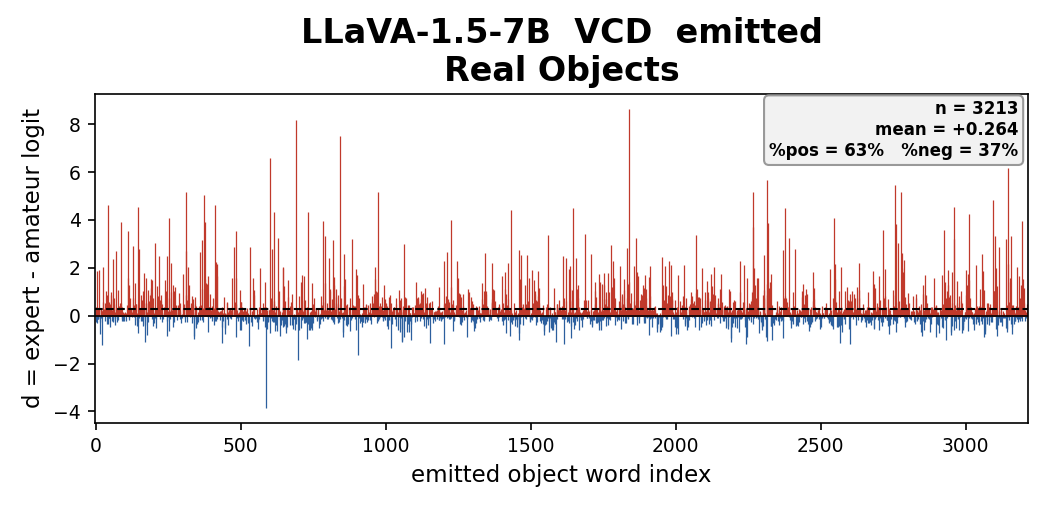
\includegraphics[width=\linewidth]{figs/llava_emit_vcd_real.png}\\[-1pt]
  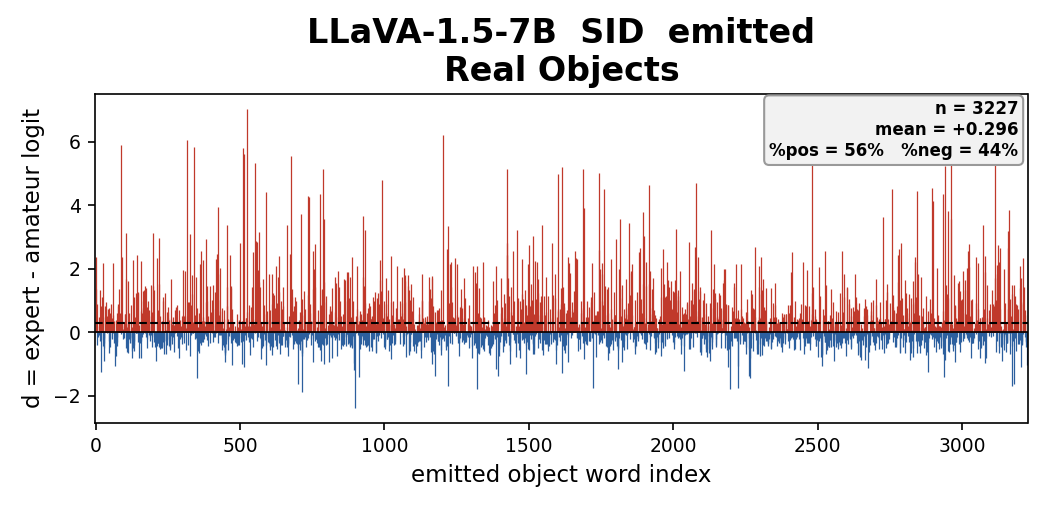
\includegraphics[width=\linewidth]{figs/llava_emit_sid_real.png}
\end{minipage}\hfill
\begin{minipage}{0.49\linewidth}\centering
  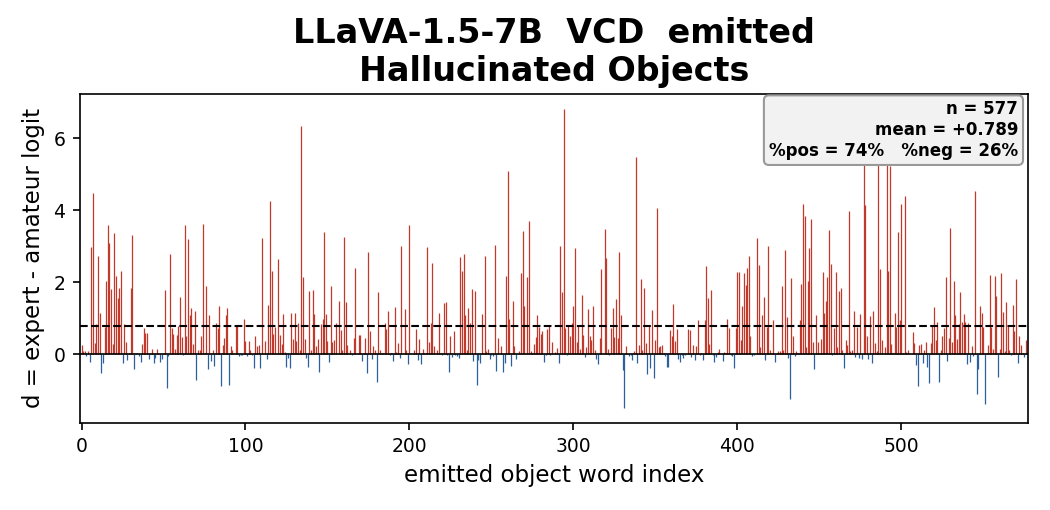
\includegraphics[width=\linewidth]{figs/llava_emit_vcd_hall.png}\\[-1pt]
  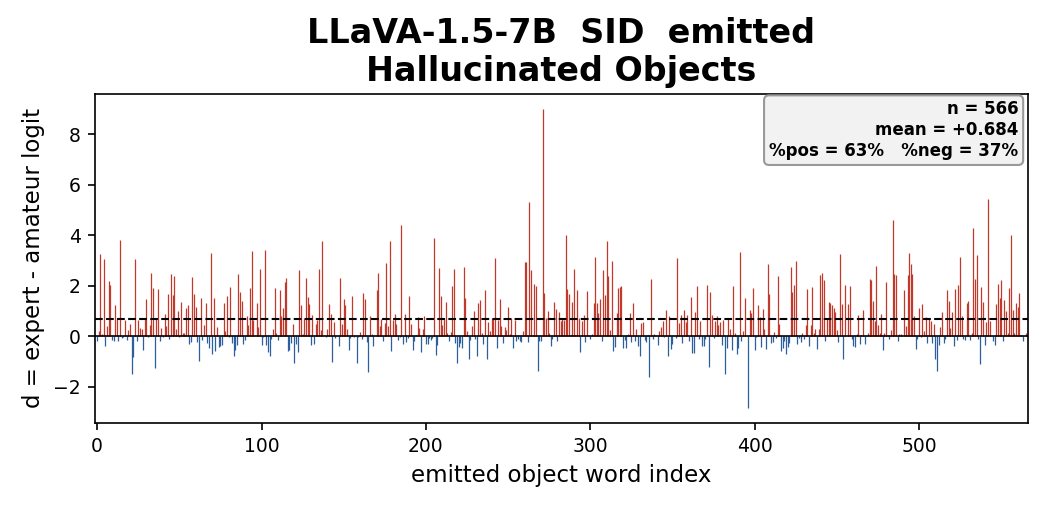
\includegraphics[width=\linewidth]{figs/llava_emit_sid_hall.png}
\end{minipage}
\caption{\textbf{LLaVA-1.5-7B: $d = E - A$ on emitted object words} (exact
caption-level labels; one thin spike per emitted word). Left column real, right
column hallucinated; top row VCD, bottom row SID. Hallucinated words are amplified
more than real words.}
\label{fig:dproxy-llava-emit}
\end{figure}

\begin{figure}[t]
\centering
\begin{minipage}{0.49\linewidth}\centering
  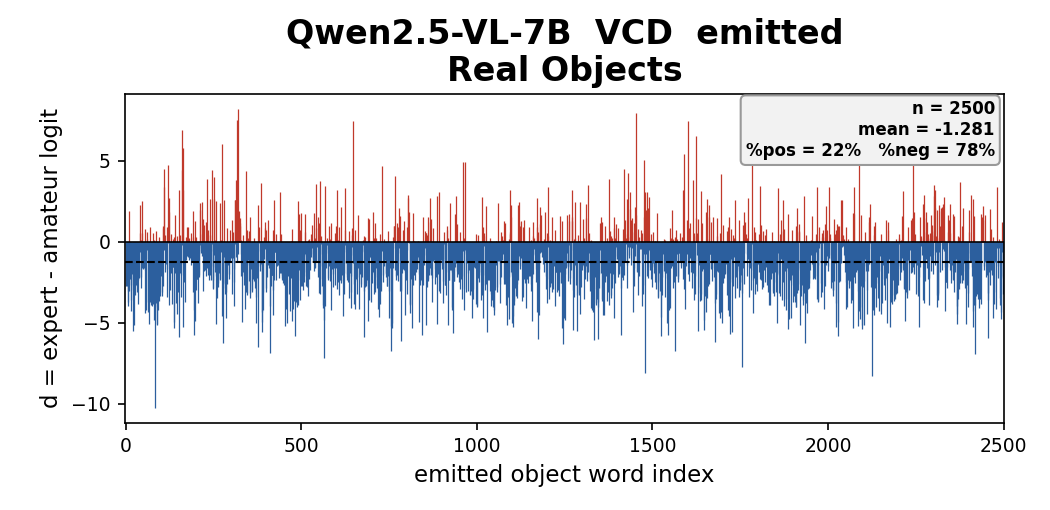
\includegraphics[width=\linewidth]{figs/qwen_emit_vcd_real.png}\\[-1pt]
  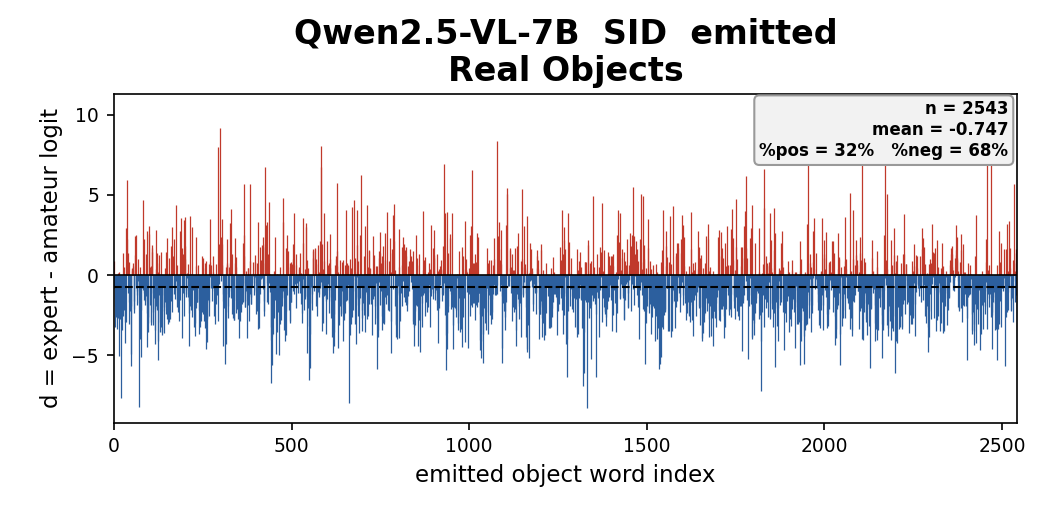
\includegraphics[width=\linewidth]{figs/qwen_emit_sid_real.png}
\end{minipage}\hfill
\begin{minipage}{0.49\linewidth}\centering
  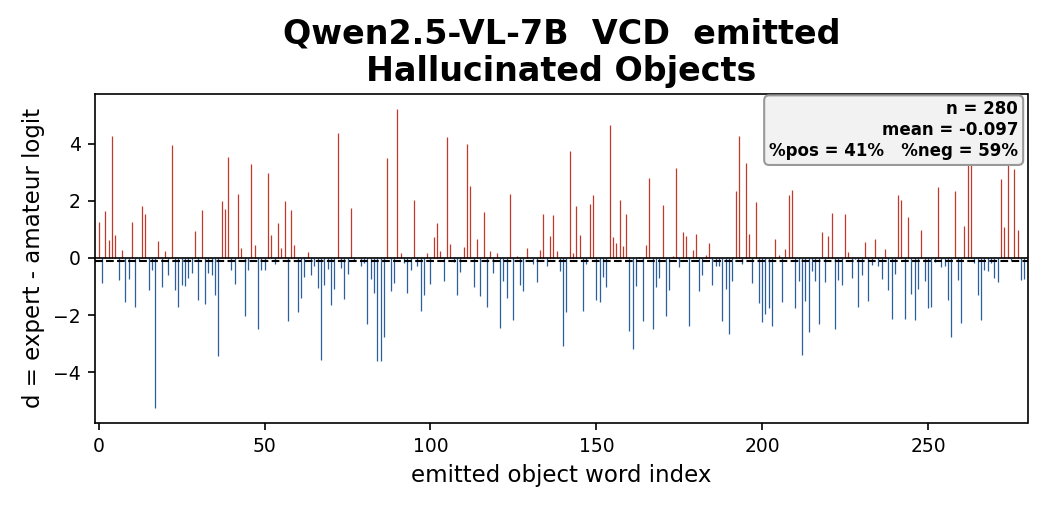
\includegraphics[width=\linewidth]{figs/qwen_emit_vcd_hall.png}\\[-1pt]
  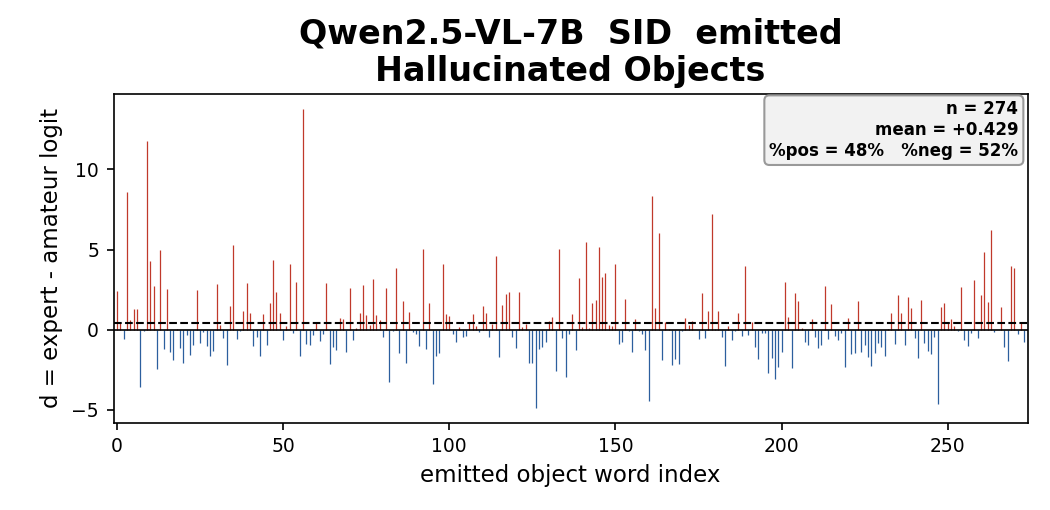
\includegraphics[width=\linewidth]{figs/qwen_emit_sid_hall.png}
\end{minipage}
\caption{\textbf{Qwen2.5-VL-7B: $d = E - A$ on emitted object words} (exact
caption-level labels; one thin spike per emitted word). Layout as in
Figure~\ref{fig:dproxy-llava-emit}. Real objects are strongly suppressed while
hallucinations sit near zero or are amplified.}
\label{fig:dproxy-qwen-emit}
\end{figure}

\textbf{Robustness across windows.} Table~\ref{tab:dproxy-robust} widens the
candidate set to the top-30. On Qwen the ordering is unchanged: hallucinated $d$
stays well above real $d$. On LLaVA both means shrink toward zero, and here
hallucinated $d$ is marginally \emph{below} real $d$ for both methods (VCD
$-0.004$ versus $+0.041$; SID $-0.018$ versus $+0.154$). These LLaVA gaps are
tiny (all $|d| \le 0.16$), and their sign is not stable: the LLaVA-SID case that
looked mildly suppressive at top-10 and top-30 reverses completely in the
exact-label emitted view below ($+0.684$ for hallucinated versus $+0.296$ for
real). We therefore do not read the small LLaVA numbers as evidence of
suppression; they are consistent with noise around zero.

\begin{table}[t]
\centering
\small
\setlength{\tabcolsep}{5pt}
\caption{\textbf{$d$ at the wider top-30 window.} Mean of $d$ over the expert's
top-30 object candidates. On LLaVA the values are near zero and the real-versus-
hallucinated ordering is not stable across windows; on Qwen hallucinated $d$
remains clearly above real $d$.}
\label{tab:dproxy-robust}
\begin{tabular}{ll cc}
\toprule
& & \multicolumn{2}{c}{Top-30 mean $d$} \\
\cmidrule(lr){3-4}
Model & Method & Real & Halluc. \\
\midrule
LLaVA-1.5-7B & VCD & $+0.041$ & $-0.004$ \\
 & SID & $+0.154$ & $-0.018$ \\
Qwen2.5-VL-7B & VCD & $-0.917$ & $-0.629$ \\
 & SID & $-0.721$ & $-0.457$ \\
\bottomrule
\end{tabular}
\end{table}

\textbf{Emitted words with exact labels.} The candidate populations rely on
single-token labels. As a co-primary check with exact caption-level labels, we
repeat the measurement on the object words the model actually emits
(Table~\ref{tab:dproxy-emitted}, and Figures~\ref{fig:dproxy-llava-emit}
and~\ref{fig:dproxy-qwen-emit}). Here the four settings agree in one direction:
emitted hallucinated objects receive a \emph{higher} adjustment than real objects
in every case (for example LLaVA-SID $+0.684$ versus $+0.296$, and Qwen-SID
$+0.429$ versus $-0.747$, where hallucinations are amplified while real objects
are suppressed). We note honestly that for LLaVA-SID this exact-label view points
the opposite way to the top-10 and top-30 candidate views: the candidate views
put hallucinated $d$ slightly below real, the emitted view puts it well above.
The two views agree only in the weak sense that neither shows the clean negative
suppression H1 predicts; they do not agree on the sign of the real-versus-
hallucinated gap for LLaVA-SID. This instability is itself the point: there is no
stable suppressive signal to be found.

\begin{table}[t]
\centering
\small
\setlength{\tabcolsep}{5pt}
\caption{\textbf{$d = E - A$ on emitted object words} (exact caption-level
labels). In every setting the emitted hallucinated adjustment is higher than the
real one, the opposite of suppression. For LLaVA-SID this reverses the sign seen
in the candidate windows (Tables~\ref{tab:dproxy-top10},~\ref{tab:dproxy-robust}),
showing the LLaVA gaps are not a stable signal.}
\label{tab:dproxy-emitted}
\begin{tabular}{ll cc cc}
\toprule
& & \multicolumn{2}{c}{Real objects} & \multicolumn{2}{c}{Hallucinated objects} \\
\cmidrule(lr){3-4}\cmidrule(lr){5-6}
Model & Method & mean $d$ & \% $d\!>\!0$ & mean $d$ & \% $d\!>\!0$ \\
\midrule
LLaVA-1.5-7B & VCD & $+0.264$ & $63.4$ & $+0.789$ & $74.0$ \\
 & SID & $+0.296$ & $56.2$ & $+0.684$ & $63.1$ \\
Qwen2.5-VL-7B & VCD & $-1.281$ & $22.0$ & $-0.097$ & $40.7$ \\
 & SID & $-0.747$ & $31.5$ & $+0.429$ & $48.2$ \\
\bottomrule
\end{tabular}
\end{table}

\subsection{Random noise of matched magnitude matches the effect on LLaVA and is exceeded by the real method on Qwen}
\label{subsec:dproxy-res-proxy}

Table~\ref{tab:dproxy-chair} reports CHAIR with image-level bootstrap $95\%$
confidence intervals, so the proxy-versus-real comparison rests on intervals
rather than single point estimates. All rows use one consistent set of runs (the
same VCD and SID runs that feed the $d$-analysis above).

On \textbf{LLaVA}, the real methods and the noise proxies have heavily
overlapping intervals on both metrics. Real VCD CHAIR-I is $15.6$ $[14.1, 17.0]$
and the two VCD noise proxies are $14.8$ $[13.3, 16.3]$ and $14.3$ $[12.9,
15.8]$; real SID is $15.1$ $[13.7, 16.6]$ and its proxies are $14.2$ and $14.5$.
The difference between real contrastive decoding and magnitude-matched random
noise is therefore within image-sampling variance. Neither real method separates
from greedy either (greedy CHAIR-I $13.9$ $[12.5, 15.3]$). In short, on LLaVA the
amateur branch does nothing to CHAIR that random noise of the same size on object
logits does not already do.

On \textbf{Qwen}, the picture is different and, for the method, worse. Real VCD
and SID raise CHAIR-I to $10.5$ $[8.9, 12.1]$ and $10.5$ $[9.1, 12.0]$, above
greedy at $7.7$ $[6.5, 8.9]$, while the noise proxies stay near greedy at $8.2$
$[6.9, 9.5]$ and $8.3$ $[7.0, 9.6]$. Here matched noise does \emph{not} reproduce
the degradation: the real subtraction pushes CHAIR up while noise of the same
magnitude leaves it near baseline. On Qwen, contrastive decoding is worse than
magnitude-matched noise, which means its harm is a structured effect of the
amateur branch, not generic perturbation.

\begin{table}[t]
\centering
\small
\setlength{\tabcolsep}{5pt}
\caption{\textbf{CHAIR for real methods versus noise proxies}, with image-level
bootstrap $95\%$ CIs ($B=10{,}000$; percentages, lower is better). Proxy A adds
Gaussian noise matched to the mean and standard deviation of $d$; Proxy B
resamples the empirical $d$ values. On LLaVA the proxy intervals overlap the real
methods; on Qwen the proxies stay near greedy while the real methods rise.}
\label{tab:dproxy-chair}
\begin{tabular}{llcc}
\toprule
Model & Setting & CHAIR-S & CHAIR-I \\
\midrule
LLaVA-1.5-7B & Greedy & $50.0$ \tiny{[45.6, 54.4]} & $13.9$ \tiny{[12.5, 15.3]} \\
 & VCD (real) & $55.0$ \tiny{[50.6, 59.4]} & $15.6$ \tiny{[14.1, 17.0]} \\
 & SID (real) & $54.2$ \tiny{[49.8, 58.6]} & $15.1$ \tiny{[13.7, 16.6]} \\
 & VCD noise proxy A & $52.4$ \tiny{[48.0, 56.6]} & $14.8$ \tiny{[13.3, 16.3]} \\
 & VCD noise proxy B & $52.8$ \tiny{[48.4, 57.2]} & $14.3$ \tiny{[12.9, 15.8]} \\
 & SID noise proxy A & $49.6$ \tiny{[45.2, 53.8]} & $14.2$ \tiny{[12.6, 15.8]} \\
 & SID noise proxy B & $50.0$ \tiny{[45.6, 54.2]} & $14.5$ \tiny{[12.9, 16.0]} \\
\midrule
Qwen2.5-VL-7B & Greedy & $30.8$ \tiny{[26.8, 34.8]} & $7.7$ \tiny{[6.5, 8.9]} \\
 & VCD (real) & $36.4$ \tiny{[32.4, 40.6]} & $10.5$ \tiny{[8.9, 12.1]} \\
 & SID (real) & $38.4$ \tiny{[34.2, 42.6]} & $10.5$ \tiny{[9.1, 12.0]} \\
 & VCD noise proxy A & $30.8$ \tiny{[26.8, 34.8]} & $8.2$ \tiny{[6.9, 9.5]} \\
 & VCD noise proxy B & $31.0$ \tiny{[27.0, 35.2]} & $8.3$ \tiny{[7.0, 9.6]} \\
\bottomrule
\end{tabular}
\end{table}

\textbf{On variance.} The intervals above capture image-sampling variance for a
single noise draw. They do not capture the variance of the random draw itself,
which would require re-running each proxy several times (a GPU cost we leave for
future work). As a rough check, two independent VCD runs on the same 500 LLaVA
images gave CHAIR-S $53.0$ and $55.0$, a gap of about two points that is
comparable to the difference between real VCD and its noise proxies. This is
consistent with the reading that, on LLaVA, real contrastive decoding and matched
noise are not distinguishable at the resolution of this experiment.

\subsection{Observations}
\label{subsec:dproxy-obs}

\begin{enumerate}
  \item \textbf{No selective suppression of hallucinations.} On Qwen,
  hallucinated objects are consistently less suppressed than real objects across
  all three populations, the opposite of the method's stated goal. On LLaVA the
  adjustments are near zero and their sign is not stable across populations, so
  they provide no evidence of suppression. H1 is clearly rejected on Qwen and
  unsupported on LLaVA; the single cell consistent with H1 (LLaVA-SID candidates)
  is negligible in size and reverses under the exact-label view.
  \item \textbf{The sign of the adjustment is model-specific.} Contrastive
  decoding amplifies object logits on LLaVA and suppresses them on Qwen. The one
  constant is that hallucinations are never suppressed more than real objects in a
  stable way.
  \item \textbf{On LLaVA the method is indistinguishable from noise.} Real and
  proxy CHAIR intervals overlap on both metrics, so the amateur branch adds
  nothing a matched random perturbation does not.
  \item \textbf{On Qwen the method is worse than noise.} Matched noise leaves
  CHAIR near greedy while the real subtraction raises it. H2 holds on Qwen, but
  not in the method's favour.
  \item \textbf{Neither method beats greedy.} On LLaVA the real methods are within
  variance of greedy; on Qwen they are clearly above it.
\end{enumerate}

\subsection{Critical analysis}
\label{subsec:dproxy-critique}

\textbf{Strengths.} The analysis targets the exact quantity the method adds to the
expert score, $d = E - A$, rather than an indirect proxy for it. It triangulates
across three populations (selection-free top-10 and top-30 candidates, and
exact-label emitted words), which is what lets us see that the LLaVA effect is
unstable rather than mistaking one window for a signal. The noise proxy is a
like-for-like control that matches the measured magnitude of $d$ and is tested in
two forms (Gaussian and empirical bootstrap) that agree, and the CHAIR comparison
now carries bootstrap intervals. Two models and two methods, on the same paired
images, guard against a single-model artifact.

\textbf{Limitations, stated plainly.} (1) The main proxy perturbs only
object-category tokens, whereas the real methods perturb the whole vocabulary. We
attempted a full-vocabulary control, but the only run available was on a 70-image
subset, and in that subset the baseline relationship itself differs from the full
sample (greedy scores above real VCD, the reverse of the 500-image result), so
the subset cannot validate the proxy's fidelity. We therefore do not report it as
evidence; a full-vocabulary proxy at 500 images, on both models, requires a GPU
run and is the clearest remaining gap. (2) The proxy CHAIR intervals capture
image-sampling variance only; noise-draw variance is estimated roughly from two
independent runs but not measured properly, which again needs repeated GPU runs.
(3) The values of $d$ are read from stored top-30 lists, so a token absent from
either list is skipped; this is rare and applies to both branches equally. (4)
The candidate populations use single-token labels, with a residual multi-word
case (for example ``bear'' from ``teddy bear'') affecting under one percent of
candidates; the emitted population has no such caveat. (5) The noise parameters
(Table~\ref{tab:dproxy-noise}) are computed over a broad pool of object tokens
that differs from the reported $d$-analysis populations, which is why their mean
does not equal any single table value; the exact pool is defined in
Section~\ref{subsec:dproxy-proxy}. (6) The Qwen SID noise proxy was not run, so
the proxy comparison covers three of the four model and method cells. (7) CHAIR
ground truth is incomplete, so an object present but neither segmented nor named
in any reference caption is scored as a hallucination; this applies identically
to every run.

\textbf{What a reviewer should take away.} The contrastive adjustment is not a
selective hallucination suppressor. On LLaVA its effect on CHAIR is
indistinguishable from matched random noise, and on Qwen it is worse than noise,
suppressing real objects more than hallucinations. This is a mechanistic account
of why the reported gains do not materialise, and it complements the
benchmark-level critique by locating the failure in the logit adjustment itself.
